%% sample template file for a MSc Thesis
%% The default is with two sided setup:
\documentclass[%
oneside,    %% uncomment for onesided layout
project,    %% uncomment not thesis but project report
nosummary   %% uncomment if no summary page should be generated
]{USN-MSc}

% The following command removes the chapter names form the header
% (comment/remove) if you prefer to have them:
\pagestyle{plain}

% --- Bibliography setup ---
%%% default is the "ieee" style
\usepackage[style=ieee, sorting=none]{biblatex}
%%% If you want to use "author-year" style
%%% where `\cite{Foo2011}` generates "Foo et al. (2011)"
%%% and   `\parencite{Foo2011}` generates "(Foo et al. 2011)"
%%% then comment the line above and use
%\usepackage[style=authoryear]{biblatex}
%%% or
%%% if you want to use "alphabetic" style then use
%%% where `cite[Foo2011]` generates "[Foo11]"
%%% then comment the line above and use
%\usepackage[style=alphabetic]{biblatex}
%%% instead.
%% load the bib file:
\addbibresource{thesis.bib}

\usepackage{lipsum} % just for providing fill text used in this template

% --- general setup ---
%% Please fill in the following parameters:
\newcommand{\mytitle}{%
%% title:
Assignment 1: Railroad predictive maintenance
}

\newcommand{\mysubtitle}{%
%% master programme (for thesis only)
%% uncomment the appropriate one:
%Electrical Power Engineering
%Energy and Environmental Technology
Industrial IT and Automation
%Process Technology
}

\newcommand{\mykeywords}{%
%% keywords (for thesis only):
<keyword one, keyword two, \ldots>
}

\newcommand{\myauthor}{%
%% author(thesis) or group code (project):
Lars Rikard Rådstoga
}

\newcommand{\myparticipants}{
%% group participants (for project only)
Lars Rikard Rådstoga
}

\newcommand{\supervisor}{%
%% supervisor:
<Supervisor's Name>}

\begin{document}

% --- title page setup ---
\USNtitlepage%
%% Please provide the following information:
%% #1 optional figure (set to {} if not wanted)
{%
  {\normalsize {}}
}
%% #2 Project partner:
{<Project partner>}
%% #3 Summary:
{%
\lipsum[6-7]
}


%\chapter*{Preface}
%\label{ch:preface}
%\addcontentsline{toc}{chapter}{Preface}
%\lipsum[1-3]
%\bigskip
%Porsgrunn, \today

%\myauthor %% for thesis
%\myparticipants %% for project


%% table of contents
\tableofcontents
\addcontentsline{toc}{chapter}{\contentsname}

%\listoffigures % out-comment if unwanted
%\addcontentsline{toc}{section}{\listfigurename}

%\listoftables  % out-comment if unwanted
%\addcontentsline{toc}{section}{\listtablename}

%\chapter*{Nomenclature}
%\label{sec:nomenclature}
%bla

%\begin{longtable}{ll}
%  \textbf{Symbol} & \textbf{Explanation}\endhead\\
%  A/D	& Analogue-Digital-Converter \\
%  CMR	& Common Mode Rejection \\
%  foo	& Foo \\
%  bar 	& Bar
%\end{longtable}

\chapter{Problem 1: Load data}
\label{ch:intro}
Data from the attached .csv file was read using a python library also called Csv.
Furthermore, the data was plotted as per instructions given by the assignment, see figure \ref{fig:raw_data_plot}.
The upper figure displays the measured acceleration data in red and the simulated data in green.
The measured signal is full of noise, but the simulated data looks to follow the general trend, or a moving average, of the measured data.
The second plot is the difference of the data, measured minus simulated. The expected behavior of this plot, that being if the measured data reflected an ideal train travelling on an ideal set of train tracks, would be evenly distributed noise.
Observing this plot as a whole, it is clear that this is not the case. Some parts of the plot, e.g. between 200 and 380 seconds looks to contain this even noise. 
But there are amplitude spikes at multiple places, most notably at ca. 190, 380 and 460 seconds. These spikes are likely due to turbulence.
\begin{figure}[!ht]
  \centering
  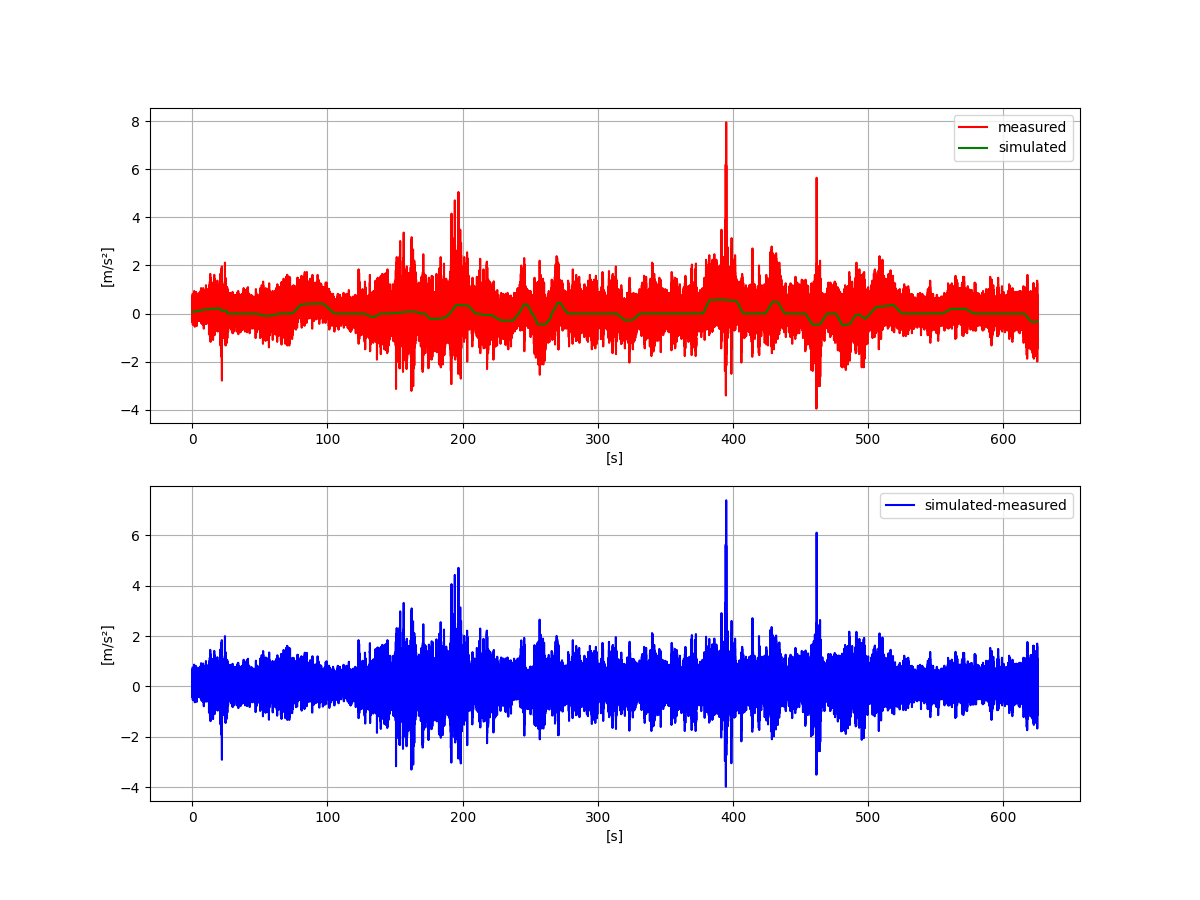
\includegraphics[width=1\textwidth]{Plotted data}
  \caption{
  A plot of the data given in the assignment. 
  The first plot shows both the measured and the simulated acceleration data. 
  And the second shows the difference between the two.}
  \label{fig:raw_data_plot}
\end{figure}

\chapter{Problem 2: FFT}
\label{ch:fft}
Both the simulated and the measured data was transformed using the FFT algorithm with the python library Numpy. The plots in figure \ref{fig:plot_meas_and_sim_fft} display the results.
The transform of the simulated data show very small amplitudes, and it is all close to 0 Hz. The measured signal, on the other hand, show both an even spread of amplitudes and bigger spikes as well.
The even spread should represent the expected noise. The spikes, especially around 3 and 38 Hz, should tell us something about non-stochastic disturbances on the system. These could be related to imperfections on the tracks, wheels, engine, and more.
My initial guess would be that the 38 Hz amplitude could be related to the wheels, according to \cite{enwiki:1105760953} the average speed of trains in Norway is 80 km/h. Quick google searches don't supply much information of wheel radii of trains in Norway.
However, another quick search says that a train moving at 72 km/h with a wheel radius of 1.2 m would have wheels with an RPM of about 160 \cite{Trainspe44:online}.
This means the wheels could be rotating at 4 times the frequency compared to this disturbance, perhaps it is still related closer to the engine, due to gears.
The 3 Hz disturbance could be related to different things, e.g. track joints in relation to lengths of the train cars. However, more information about the train and the track are needed to say for sure.

\begin{figure}[!ht]
  \centering
  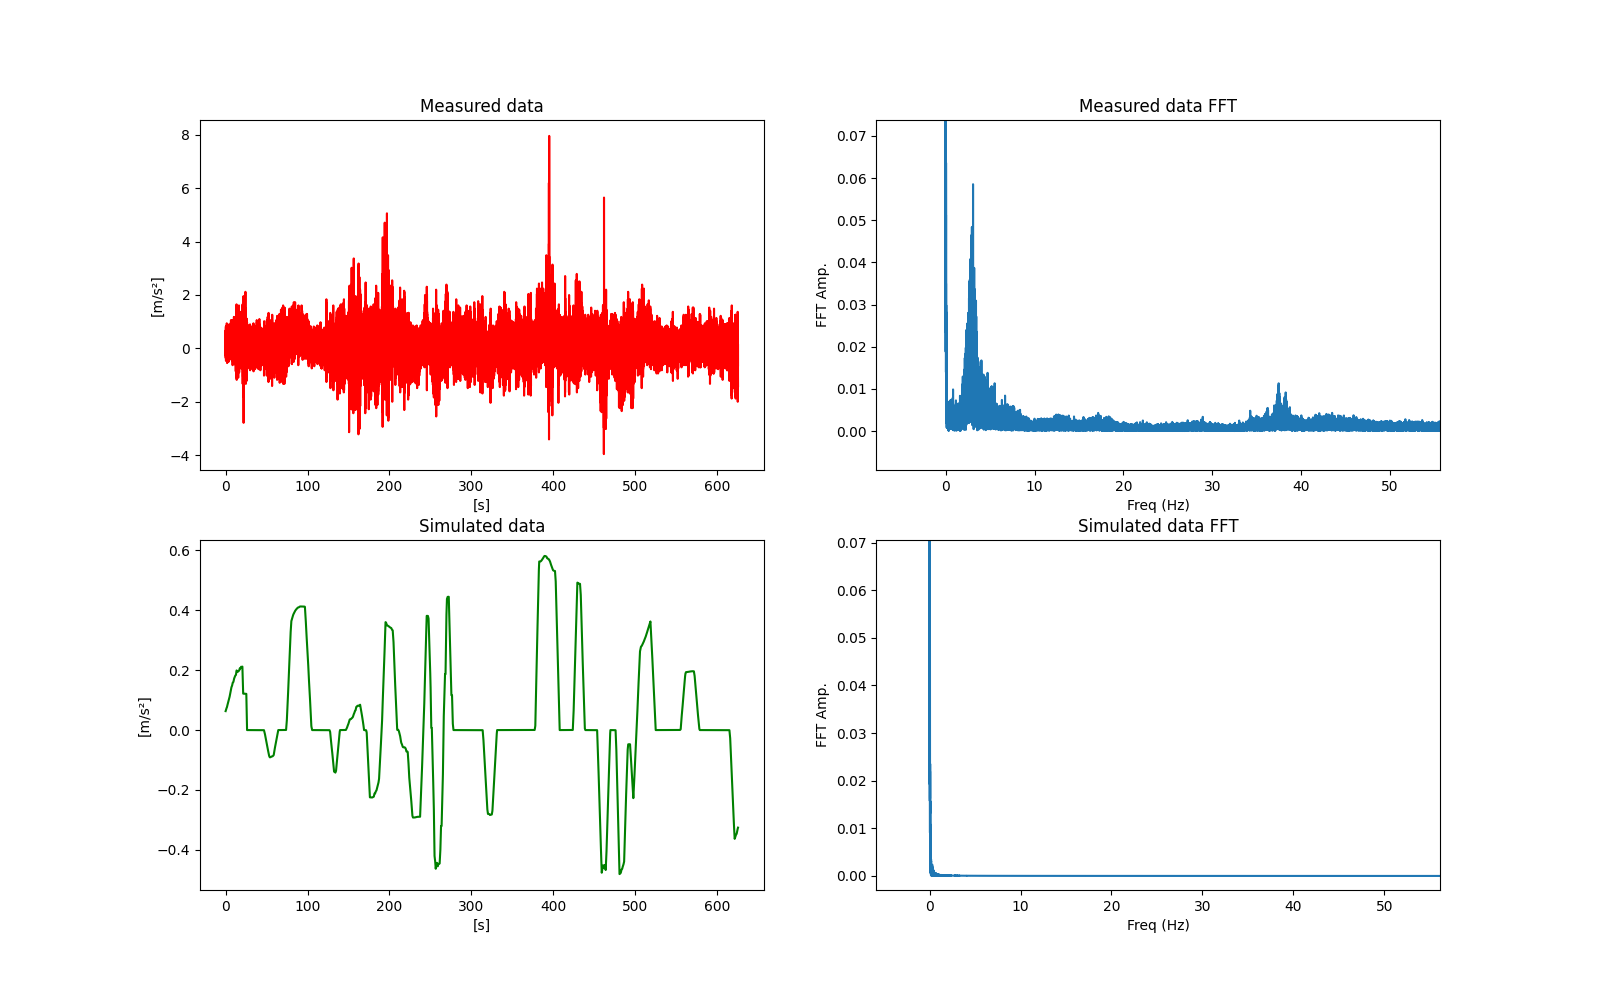
\includegraphics[width=1\textwidth]{Plotted Measured and Simulated FFT}
  \caption{
  A plot of both the original data, measured and simulated data on the left and their respective FFT plots in the frequency domain on the right.}
  \label{fig:plot_meas_and_sim_fft}
\end{figure}

\chapter{Problem 3: Comparing model with measurements}
\label{ch:comparison}
The difference between the measured and simulated data was transformed using the FFT algorithm and plotted in figure \ref{fig:plot_diff_fft} together with the non-transformed data. There isn't any noticeable difference that I can point out.

\begin{figure}[!ht]
  \centering
  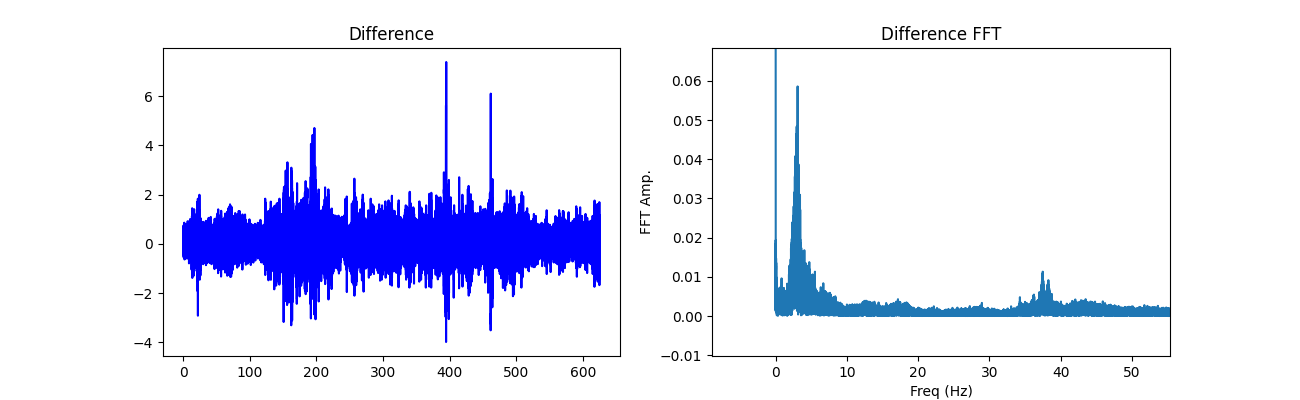
\includegraphics[width=1\textwidth]{Plotted difference FFT}
  \caption{
  Plot of the difference in data: measured - simulated. Original data on the left and transformed using the FFT algorithm on the right.}
  \label{fig:plot_diff_fft}
\end{figure}

% A dummy command that causes all bibliographyentries to be displayed
% even though there were not cited in the document. Used for demonstration
% purposes only in this template file.
~\nocite{*}

\cleardoublepage

% The bibliography should be displayed here...
%\printbibliography[heading=bibintoc]
% You rather like to call the bibliography "References"? Then use this instead:
\printbibliography[heading=bibintoc, title={References}]


%\appendix
%%\renewcommand{\appendixname}{Paper} %% So we get 'Paper X' displayed instead
%
%
%\chapter[Short Title of Paper A]{Title of Paper A (probably very long and therefore not good to have in the header)}
%\label{paper-a}
%
%\paragraph{Note}
%Since some papers tend to have a rather long title it is good to provide the optional short title which then will be displayed in the table of contents and header instead of the long original title.
%On the openening page of the chapter the orginal \emph{long} title will be displayed.\bigskip
%
%\emph{Short descriptive text of paper follows here.}\bigskip
%
%The paper itself needs to be included in the published form as PDF on the next pages.
%This can be done using the \texttt{pdfpages} package by adding the command:
%
%\begin{verbatim}
%\includepdf{pages=-,openright}{Filename}
%\end{verbatim}
%
%You can omit the \texttt{.pdf} when specifying the \texttt{Filename}. Also you should include always include the option \texttt{openright} since it would look strange to have the paper starting at the back of the cover page.
%
%There are more options like only adding specific pages:
%\begin{verbatim}
%\includepdf{pages=2-6,openright}{Filename.pdf}
%\end{verbatim}
%
%For more options see Appendix~\ref{paper-b} where the most important pages of the \texttt{pdfpages} manual were inlcuded using \texttt{pdfpages}.
%
%
%%%% Command to include a PDF file directly including all pages:
%
%
%\chapter[Short Title of Paper B]{Title of Paper B}
%\label{paper-b}
%Short descriptive text of paper follows here.
%
%Here we included the first five pages of the \texttt{pdfpages} manual itself.
%
%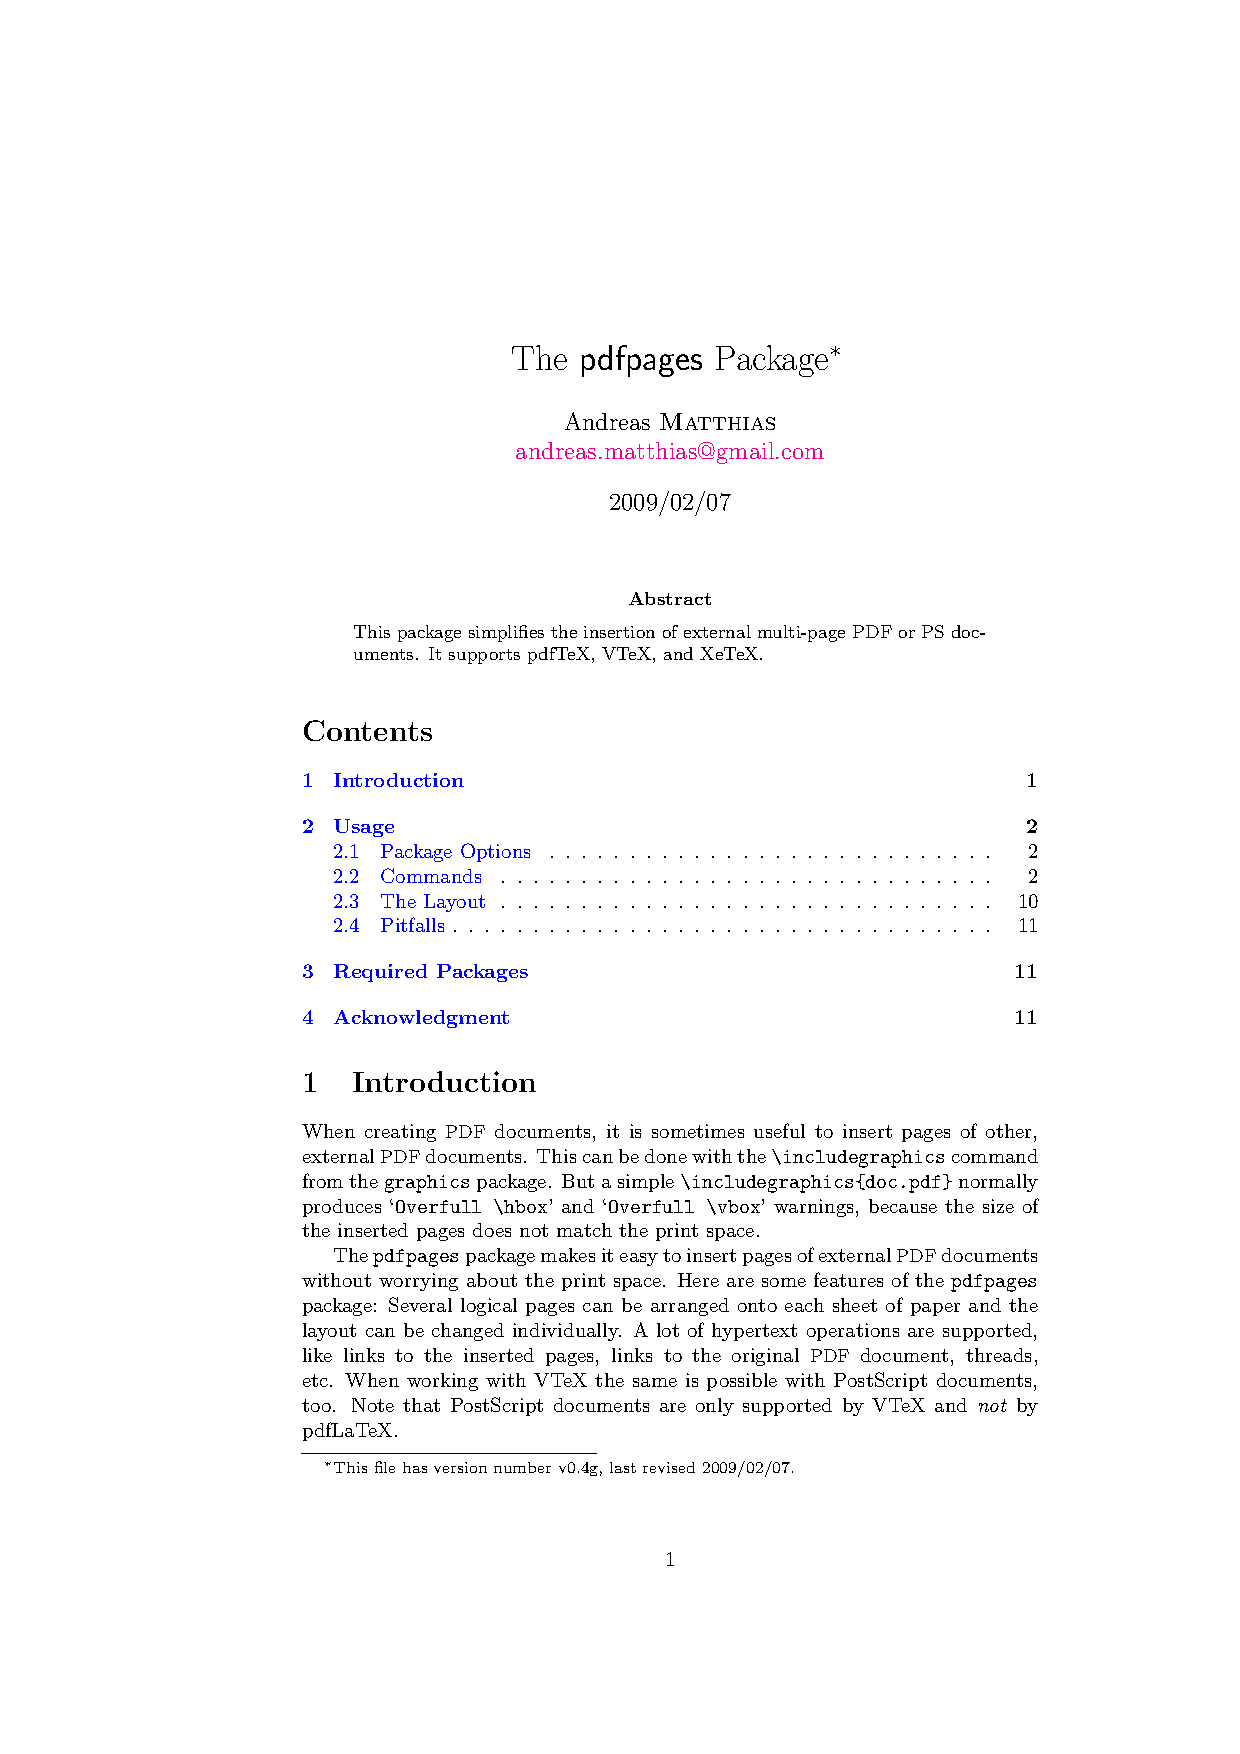
\includepdf[pages=1-5,openright]{fig/pdfpages}

\end{document}

%%% Local Variables:
%%% mode: latex
%%% TeX-master: t
%%% End:
